\documentclass[main]{subfiles}


\begin{document}

\chapter{Caracterizaci\'on de los motores y las h\'elices}\
\label{chap:test_motores}
\section{Objetivo}
El objetivo es el de caracterizar los motores del cuadric\'optero Turbo Ace X720. Se busca:

\begin{itemize}
\item Analizar el comportamiento de los cuatro motores individualmente
\item Determinar la relaci\'on entre velocidad angular y fuerza
\item Determinar la relaci\'on entre comando $I^2C$ y la velocidad angular.
\item Determinar la relaci\'on entre velocidad angular y torque.
\item Determinar la respuesta al escal\'on
\end{itemize}

Los algoritmos de control se encargan de definir la velocidad angular de los motores en cada instante, por dicho motivo es fundamental conocer la relaci\'on que existe entre esta \'ultima y la fuerza y el torque que se produce. La principal ventaja de esta elecci\'on es que el lazo de control implementado es independiente de la tecnolog\'ia utilizada en el control de los motores ($I^2C$, PWM,etc) y por ende permite la reutilizaci\'on del mismo. Dado que actualmente el control de los motores se establece mediante un comando $I^2C$ es fundamental comprender la relaci\'on que existe entre este comando y la velocidad angular.

\section{Materiales}
\begin{itemize}
\item Cuadric\'optero Turbo Ace X720	
\item LED IR TSAL6200
\item Detector IR TSOP38256
\item Resistencia de $20 \Omega$
\item Generador de onda Tektronix CFG250
\item Fuente de alimentaci\'on de $5V_{DC}$
\item Osciloscopio digital GwINSTEC GDS2062
\item Balanza Presiser LK-15P presici\'on media III
\item Beagleboard XM rev C
\item Analizador l\'ogico ChronoVu
\item Buffer Octal 74HC245
\end{itemize}


\section{Procedimiento}


\subsection{Consideraciones previas}
\label{sec:test_motores--disp-forma-u}

El detector IR TSOP38256 es sensible a radiaciones infrarrojas moduladas a una frecuencia de $56$ KHz. Si se lo expone a una onda cuadrada de dicha frecuencia la salida del mismo es un ``0'' l\'ogico. Si no recibe dicha radiaci\'on la salida es un ``1'' l\'ogico.\\
\begin{wrapfigure}{r}{0.55\textwidth}
  \begin{center}
    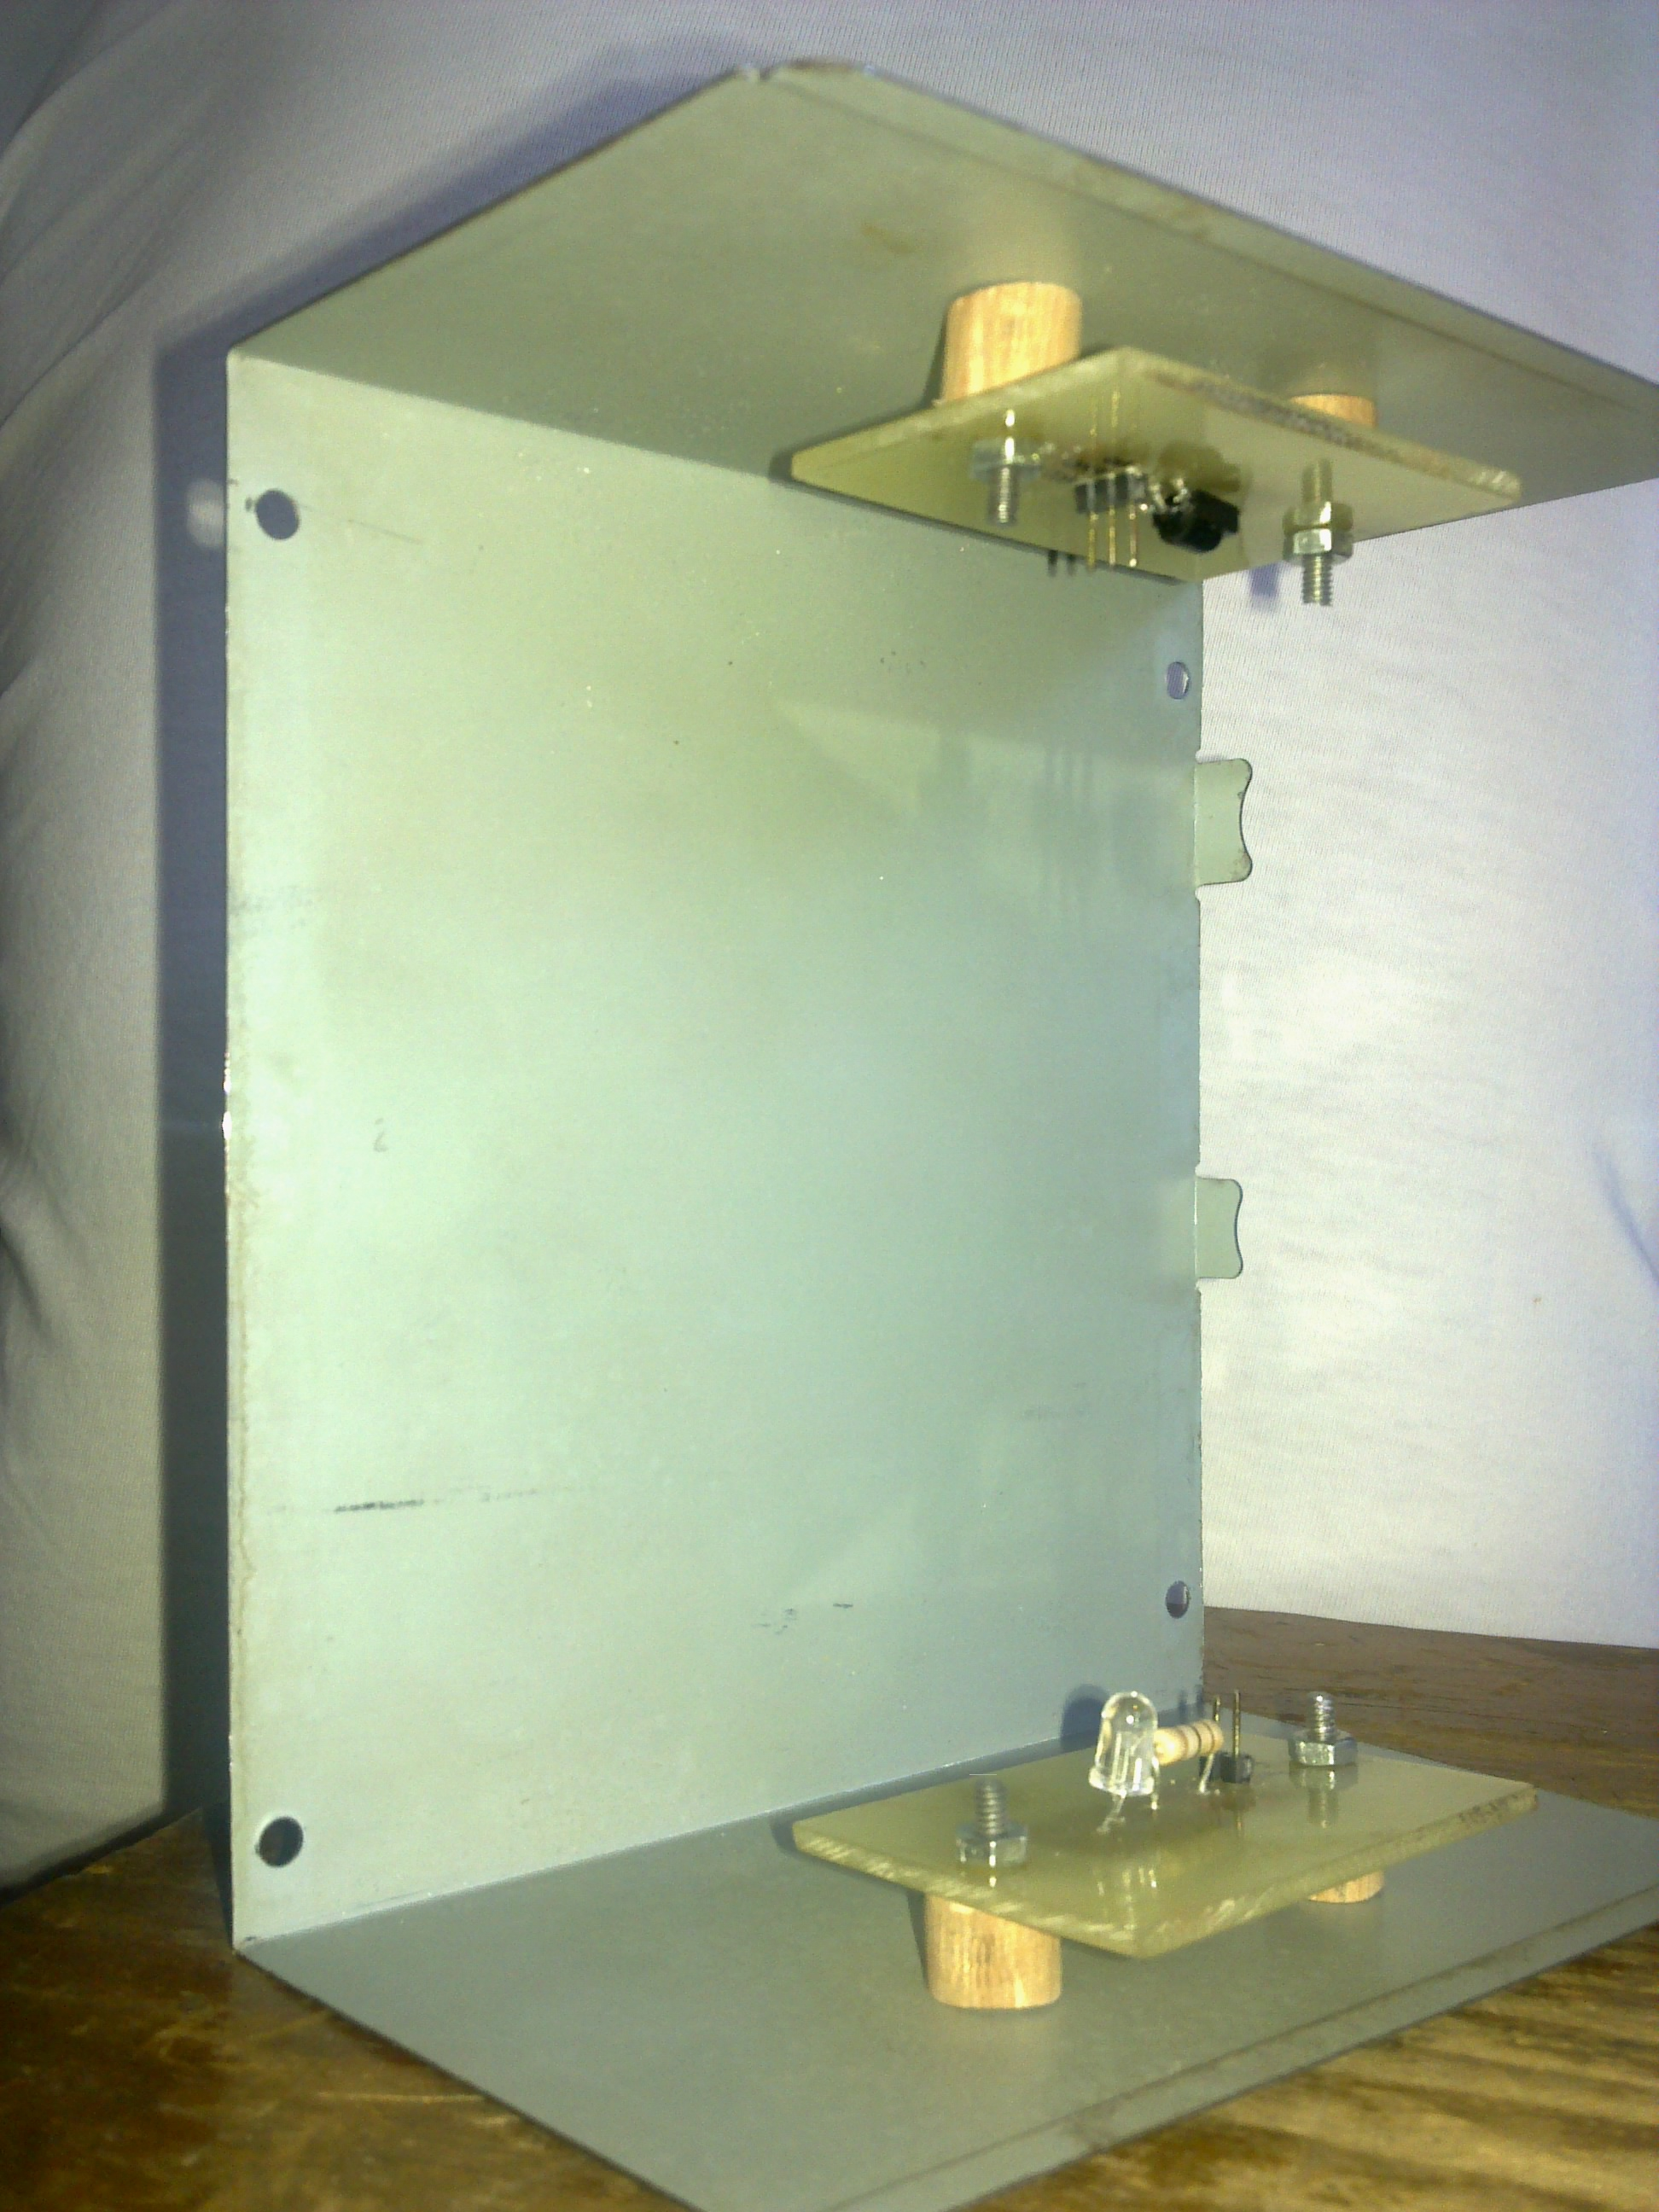
\includegraphics[width=0.25\textwidth]{./pics_motores/u.jpg}
  \end{center}
  \caption{Dispositivo en forma de U}
  \label{fig:u}
\end{wrapfigure}
El dispositivo de medida de velocidad angular se trata de un cuerpo en forma de ``U", de un lado se tiene el LED infrarrojo y del otro el detector, tal como se puede ver en la figura \ref{fig:u}.
La idea del dispositivo de medida es sencilla. Se trata de hacer ``pasar'' la radiaci\'on infrarroja emitida por el LED a trav\'es de la h\'elice en funcionamiento de uno de los motores. Esta radiaci\'on es recogida del otro lado por el receptor IR. De este modo tendremos a la salida del detector, pulsos de frecuencia correspondientes a la velocidad con la que la h\'elice obstruye el camino entre el sensor y el LED. \textbf{La velocidad angular ser\'a entonces la mitad de dicha frecuencia}.\\

\begin{wrapfigure}{l}{0.4\textwidth}
  \begin{center}
  \vspace{-20pt}
    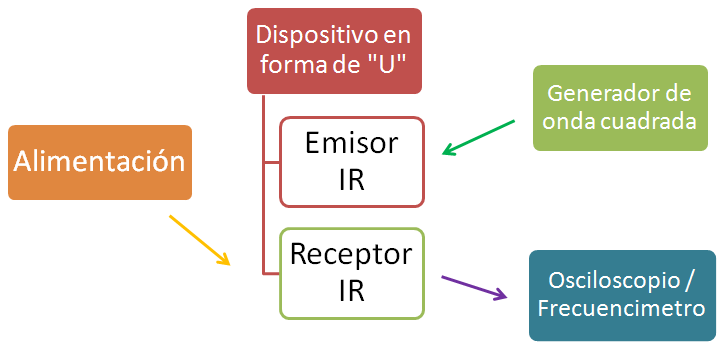
\includegraphics[width=0.35\textwidth]{./pics_motores/dispositivoU.png}
  \end{center}
  \vspace{-10pt}
  \caption{Diagrama \\de interconexión}
    \vspace{-10pt}
  \label{fig:diagrama_u}
\end{wrapfigure}

Como explicamos anteriormente el LED debe ser conmutado con una frecuencia de 56kHz por lo tanto se lo alimentar\'a con un generador de se\~nales funcionando como generador de onda cuadrada a dicha frecuencia. Para lograr un correcto funcionamiento del LED se requiere una corriente superior a los $100mA$. La amplitud de la onda cuadrada se regular\'a a $5V$ y se trabajar\'a con una resistencia de $20\Omega$ en serie. La salida del receptor IR se conecta directamente al osciloscopio digital, el cual es capaz de medir frecuencias. El diagrama de interconexión puede apreciarse en la figura \ref{fig:diagrama_u}.\\

\subsection{Relaci\'on entre comando $I^2C$, velocidad angular y empuje}

\subsubsection*{Obetivos particulares}
Este experimento servir\'a para relevar:
\begin{itemize}
\item Diferencias en el comportamiento de los motores
\item Relaci\'on entre velocidad angular y fuerza
\item Relaci\'on entre comando $I^2C$ y la velocidad angular.
\end{itemize}

\subsubsection*{Modelos de ajuste}

Si no se env\'ia ning\'un comando $I^2C$ los motores no giran. Es evidente que si los motores no giran las h\'elices no realizan ning\'un empuje. Por lo tanto los modelos deben ``pasar'' por el origen. 
\begin{itemize}


\item Para la relaci\'on entre velocidad angular y fuerza, en base a \cite{bib:fuerzas-helices}, se proponen los siguientes modelos de ajuste:

	\begin{itemize}
	\item Modelo cuadr\'atico $T=a\omega^2+b\omega$
	\item Modelo c\'ubico $T=a\prime \omega^3+b\prime \omega^2+c\prime$
	\end{itemize}

\item Para la relaci\'on entre velocidad angular y comando $I^2C$ se proponen los siguientes modelos de ajuste:
	\begin{itemize}
	\item Modelo cuadr\'atico $x=a\omega^2+b\omega$
	\item Modelo c\'ubico $x =a\prime \omega^3+b\prime \omega^2+c\omega$	
	
	\end{itemize}


\end{itemize}

\subsubsection*{Desarrollo del experimento}
El procedimiento consiste en enviar distintos comandos $I^2C$ al cuadric\'optero y registrar las diferentes lecturas de masa en la balanza para determinar el empuje de los motores y en registrar las diferentes medidas de frecuencia en el osciloscopio para determinar la velocidad angular de los cuatro motores.
El setup experimental puede observarse en la figura \ref{fig:setup1}.
Se solidariza el cuadric\'optero a una base de madera. Sobre esta \'ultima se a\~nade peso suficiente para asegurar que el cuadric\'optero no se eleve, se agregaron 3Kg de sobrepeso.


	
Al estar el sistema en equilibrio mec\'anico se cumple que:
\begin{equation}
\sum F_{ext}=0
\end{equation}

En este caso las fuerzas presentes son el peso del sistema ($M_{total}g$) la normal de la balanza sobre el sistema ($N=N_1+N_2$) y el empuje de los motores ($T_{total}=T_1+T_2+T_3+T_4$). Por lo tanto:
\begin{equation}
T_{total}-M_{total}g+N=0
\end{equation}\\

\begin{wrapfigure}{l}{0.45\textwidth}
\vspace{-25pt}
  \begin{center}
    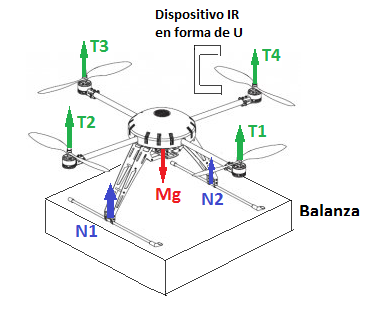
\includegraphics[width=0.35\textwidth]{./pics_motores/set1.png}
  \end{center}
  \vspace{-25pt}
  \caption{Primer set-up\\ experimental}
  \label{fig:setup1}
\end{wrapfigure}

Por lo tanto el empuje de los motores puede calcularse como:
\begin{equation}
T_{total}=M_{total}g-N
\end{equation}

La lectura de la balanza no es otra cosa que $\frac{N}{g}$.
Una vez ubicado el cuadric\'optero con el sobrepeso sobre la balanza se tara la balanza. Por lo tanto la lectura que indica la balanza($M_{medida}$) luego de realizada esta acci\'on es:
\begin{equation}
M_{medida}=\frac{N-M_{total}g}{g}
\end{equation}

Por lo tanto el empuje de los cuatro motores puede calcularse como:

\begin{equation}
T_{total}=-M_{medida}g
\end{equation}
Asumiendo que los cuatro motores se comportan en forma similar se tiene que:

\begin{equation}
T=-\frac{M_{medida}g}{4}
\end{equation}

La medida de frecuencia se realiza con el dispositivo IR descripto en la secci\'on anterior. La frecuencia medida ($f_{medida}$) corresponde al inverso del tiempo que transcurre entre el pasaje de una hoja de la h\'elice y la otra. El per\'iodo de la rotaci\'on de la h\'elice es el doble y por ende la frecuencia de la rotaci\'on es la mitad de la frecuencia medida. Por lo tanto se tiene que:
\begin{equation}
\label{eq:omega_ir}
\omega=2\pi f=\pi f_{medida}
\end{equation}

Se mide la velocidad angular de los cuatro motores y se trabaja con el promedio. En la secci\'on \ref{sec:motores} se ver\'a porqu\'e es adecuado considerar el promedio.

\subsection{Relaci\'on entre velocidad angular y torque}

\subsubsection*{Objetivos espec\'ificos}
El objetivo de este experimento es obtener la relaci\'on entre velocidad angular y torque.

\subsubsection*{Modelos de ajuste}
Nuevamente el modelo se fuerza para obtener un torque nulo a velocidad angular nula. De acuerdo al an\'alisis realizado en \ref{chap:modelo} se propone un modelo cuadr\'atico:

$$Q=a\omega^2+b\omega$$

\subsubsection*{Desarrollo del experimento}
\label{sub:torque}
Se ubica el cuadric\'optero sobre la balanza. Se retiran tres de las cuatro h\'elices del cuadric\'optero. La cuarta h\'elice se rota de forma que su eje principal se encuentre paralelo al plano de la balanza. Se ubica el detector IR de forma de poder medir la velocidad angular de la h\'elice. El setup de medida puede verse en la figura \ref{fig:setup2}. De acuerdo a lo estudiado la h\'elice presenta un torque ($Q$) negativo respecto de su eje central si el motor rota en sentido anti-horario. Nos proponemos calcular el torque total respecto de dicho eje. Las fuerzas presentes en el sistema son: el peso, la fuerza de empuje, la resultante de las normales ($N = N1+N2$) y las fuerzas de fricci\'on en el plano del plato de la balanza. Estas \'ultimas y el empuje no realizan ning\'un torque en la direcci\'on de inter\'es. Recordamos que el torque de una fuerza respecto de un eje se calcula como:
\begin{wrapfigure}{l}{0.55\textwidth}
  \vspace{0pt}
  \begin{center}
    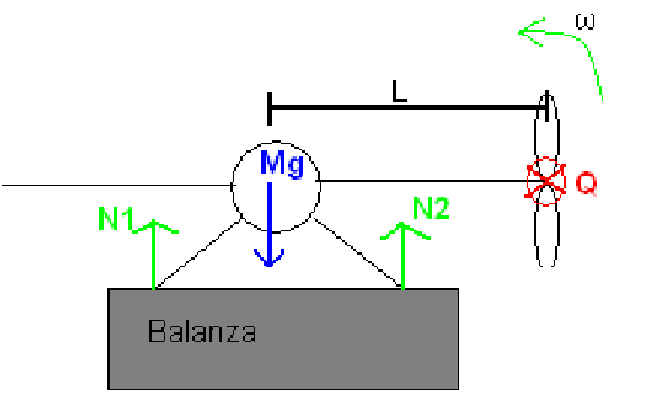
\includegraphics[width=0.45\textwidth]{./pics_motores/set2.pdf}
  \end{center}
  \vspace{-15pt}
  \caption{Segundo set-up experimental}
  \label{fig:setup2}
  \vspace{10pt}
\end{wrapfigure}
\begin{equation}
\tau=\vec{r} \times \vec{F} 
\end{equation}

Donde $\vec{F}$ es la fuerza considerada y $\vec{r}$ es vector distancia entre el eje y el punto de aplicaci\'on de la fuerza.\\

Definimos el largo $L=29.3cm$ como la distancia entre el eje de la h\'elice y el centro de masa del cuadric\'optero. El peso se aplica en el centro de masa y se asume por simetr\'ia que la resultante de las normales se aplica sobre la recta que pasa por el centro de masa del cuadric\'optero y es perpendicular a la balanza. 

De esta forma se tiene que el torque total vale:
\begin{equation}
\tau = -Q+LM_{total}g-LN=-Q+L(M_{total}g-N)
\end{equation}

Como se explico anteriormente luego de tarar la balanza la masa medida por la misma corresponde a $M_{medida}=\frac{N-M_{total}g}{g} $. De esta forma se puede escribir el torque total como:
\begin{equation}
\tau=-Q-LM_{medida}g
\end{equation}
Al igual que en el experimento anterior el sistema se encuentra en equilibrio mec\'anico y por lo tanto: 
\begin{equation}
\tau=0
\end{equation}

De esta forma queda claro que el torque que nos interesa caracterizar puede calcularse como:
\begin{equation}
Q=-LM_{medida}g
\end{equation}

\subsection{Respuesta al Escal\'on}
Se caracterizar\'a al motor en lo que respecta a su respuesta al escal\'on. Se ver\'a cuanto demora un motor en pasar de la velocidad angular en r\'egimen correspondiente al valor de comando $I^2C$ 50 a la velocidad angular en r\'egimen correspondiente al valor de comando $I^2C$ 150. El osciloscopio no resulta adecuado para observar las diferencias de velocidad angular obtenidas. Se procede a conectar la salida del sensor IR a un \emph{buffer} octal y la salida de este \'ultimo al analizador l\'ogico\footnote{ Esto fue necesario ya que la tensi\'on de la salida del IR disminu\'ia dr\'asticamente al conectarlo directamente al analizador l\'ogico a valores que este \'ultimo no es capaz de identificar como ``1'' l\'ogicos.}. El analizador l\'ogico registra la salida del sensor IR durante 5 segundos a una tasa de muestreo de 2kHz. Se obtendr\'an las diferencias de tiempos entre flancos de subida sucesivos($t_f$). Cada flanco de subida corresponde a una hoja de la h\'elice siendo detectada por el sensor IR. La velocidad angular de la h\'elice puede calcularse como:

\begin{equation}
\omega = 2 \pi \frac{1}{2t_f} = \frac{\pi}{t_f}
\end{equation}
 
\section{Resultados y an\'alisis}

\subsection{Comparaci\'on entre motores}
\label{sec:motores} 

En la tabla \ref{tab:motores} se presentan los resultados obtenidos experimentalmente de acuerdo al procedimiento descrito. 


\begin{table}[H]
\centering
\begin{tabular}{|c|c|c|c|c|c|} 
	\cline{3-6} \multicolumn{1}{c}{} & \multicolumn{1}{c}{} & 
	\multicolumn{4}{|c|}{\cellcolor[gray]{0.6}Frecuencia (Hz)} \\ \hline
	\cellcolor[gray]{0.8} {$\mathbf{I^2C}$} & 
	\cellcolor[gray]{0.8} \textbf{Peso medido (g)} &
	\cellcolor[gray]{0.8} \textbf{Motor D0} &
	\cellcolor[gray]{0.8} \textbf{Motor D2} &
	\cellcolor[gray]{0.8} \textbf{Motor D4} &
	\cellcolor[gray]{0.8} \textbf{Motor D6}   \\ \hline \hline
	  0 &      0 &    0 &    0 &    0 &    0 \\ \hline
	 50 &-165 & 34.2 & 34.3 & 35.5 & 34.3 \\ \hline
	 70 &-360 & 49.2 & 49.5 &   49 & 48.4 \\ \hline
	 90 & -590 & 63.7 & 62.7 & 63.3 & 63.5 \\ \hline
	110 & -865 & 76.7 & 74.4 & 75.5 & 73.4 \\ \hline
	130 &  -1120 & 87.3 & 86.3 & 86.2 & 84.7 \\ \hline
	150 & -1395 & 97.5 & 95.4 & 96.2 & 94.2 \\ \hline
	170 & -2030 &104.7 &104.2 &106.2 &105.5 \\ \hline
	200 & -2535 &115.5 &113.4 &119.9 &117.3 \\ \hline
\end{tabular}
\caption{Comando $I^2C$ enviado, peso medido y frecuencia medida para los cuatro motores}
\label{tab:motores}
\end{table}

En la figura \ref{fig:motores} se presentan las velocidades angulares de los cuatro motores contra el comando $I^2C$, mientras que en la figura \ref{fig:difmotores} se muestra la diferencia entre la velocidad angular de cada motor y el promedio de las mismas para cada comando $I^2C$ enviado. En la figura \ref{fig:motores} se observa que el comportamiento de los motores es en todos los casos similar. Para velocidades angulares bajas los motores se comportan en forma id\'entica y lineal, y comienzan a distanciarse al aumentar la velocidad.\\
 

\begin{figure}[h!]
  \begin{center}
	\subfloat[Velocidad angular de los cuatro motores]{\label{fig:motores}
	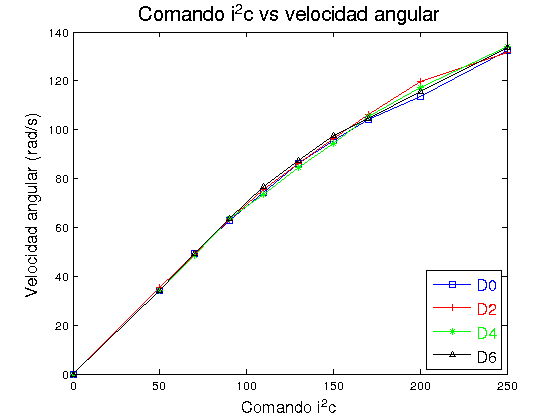
\includegraphics[width=0.5\textwidth]
		{./pics_motores/motores.png}}
	\subfloat[Error en la velocidad angular de los cuatro motores]{\label{fig:difmotores}
	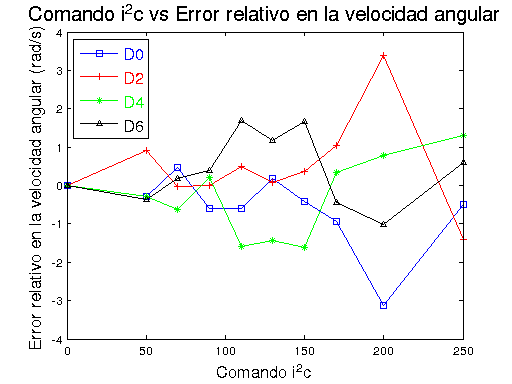
\includegraphics[width=0.5\textwidth]
		{./pics_motores/difmotores.png}}
		
  \end{center}
  \caption{Curva $I^2C$ vs. velocidad angular para los 4 motores}

\end{figure}

En la figura \ref{fig:difmotores} puede observarse que la m\'axima diferencia entre las velocidades angulares de dos motores es de aproximadamente $6.5 rad/s$. Dicha diferencia se obtiene para un valor de comando $I^2C$ igual a 200. Si observamos la velocidad angular a dicho valor de comando $I^2C$ en la tabla \ref{tab:motores} se observa que el menor valor corresponde a $113.4 rad/s$. El error relativo que se obtiene es inferior al $6\%$


Se puede afirmar que:
\begin{itemize}
\item Es v\'alido promediar las velocidades angulares de los 4 motores y trabajar con esos promedios como un motor típico. Adem\'as de este modo se reducen los posibles errores que se pueden haber causado a la hora de realizar las medidas.
\item Por lo tanto la fuerza medida (de los 4 motores juntos) corresponde con el cu\'adruple de la fuerza ejercida por cada uno de ellos
\end{itemize}


\subsection{Obtenci\'on de la curva fuerza contra velocidad angular}

Se trabaja con la medida de peso presentada en la tabla \ref{tab:motores} y con el promedio de las medidas de la frecuencia de dicha tabla.\footnote{De acuerdo a las justificaciones realizadas en la secci\'on \ref{sec:motores}}. En la figura \ref{fig:fvel} se observan los puntos obtenidos experimentalmente y las curvas obtenidas con los modelos de ajuste propuestos. En dicha figura se observa que ambos modelos aproximan adecuadamente los puntos obtenidos experimentalmente.\\

Para el modelo cuadr\'atico se obtiene:
\begin{itemize}
\item Par\'ametros: \newline$a=4.6016\times10^{-5}Ns^2$,\newline$b=-1.0380\times 10^{-3}Ns$
\item Error promedio: \newline$e=-3.9951\times 10 ^{-4}N$,\newline $e=-0.4072\times 10 ^{-1}g$
\item Desviaci\'on est\'andar :\newline$\sigma=2.3871\times10^{-2}N$,\newline $\sigma=2.4333g$
\end{itemize}

Para el modelo c\'ubico se obtiene:
\begin{itemize}
\item Par\'ametros:\newline$a\prime = 3.0619\times 10^{-9}Ns^3$,\newline$b\prime =4.1319\times10^{-5}Ns^2$,\newline$c\prime -3.9160\times10^{-4}Ns$
\item Error:\newline $e =-1.4331\times10^{-4}N$, \newline $e=-0.1461g$
\item Desviaci\'on est\'andar: \newline $\sigma=2.3377\times 10^{-2}N$, \newline $\sigma =2.3830g$
\end{itemize}

El c\'alculo del error promedio y la desviaci\'on est\'andar no presenta diferencias significativas para uno y otro modelo, por lo tanto se opta por trabajar con el modelo m\'as sencillo, es decir el cuadr\'atico. Asimismo el error obtenido es despreciable respecto de la resoluci\'on de la balanza y la desviaci\'on est\'andar es del \'orden de la presici\'on de la misma, por lo que se consluye que la caracterizaci\'on es satisfcatoria. Se tiene entonces que:
\begin{equation}
T=4.6016\times10^{-5}\omega^2-1.0380\times10^{-3}\omega
\end{equation}
Con $\omega$ en $rad/s$ y $T$ en $N$.
\begin{figure}[H]
  \vspace{-20pt}
\hspace{-50pt}
\subfloat[Curva experimental de Fuerza-Velocidad angular]{\label{fig:fvel}
  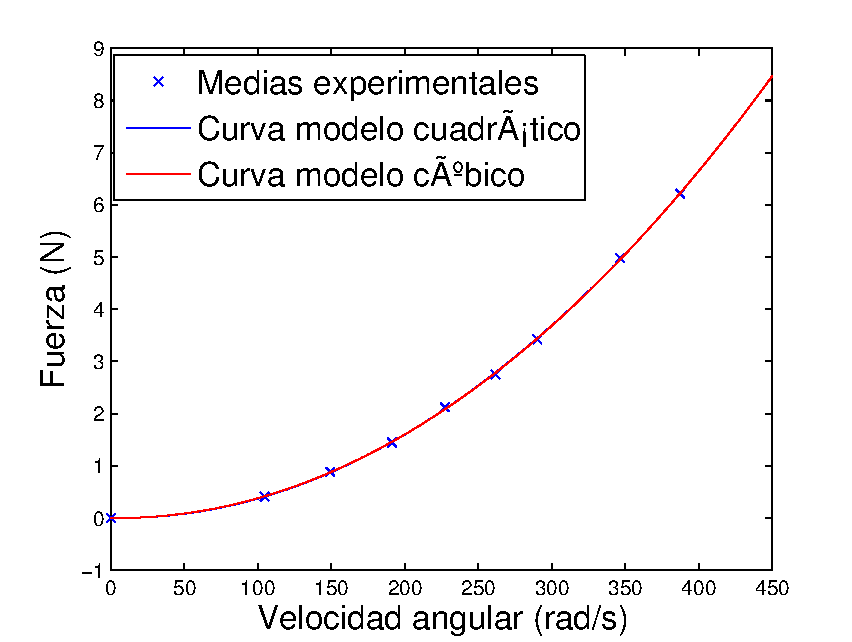
\includegraphics[width=0.6\textwidth]{./pics_motores/fvel.pdf}}
\subfloat[Curva $I^2C$ en funci\'on de la velocidad angular]{\label{fig:iwi}
  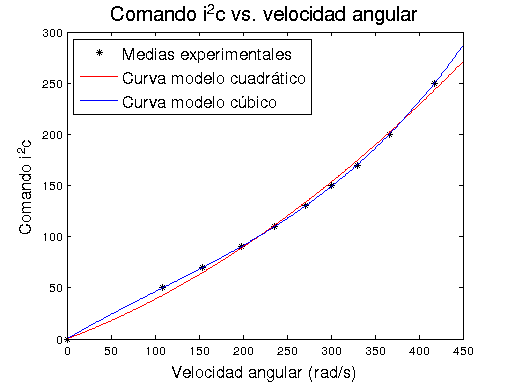
\includegraphics[width=.6\textwidth]{./pics_motores/wi.png}}
  \vspace{-5pt}
  \caption{}  
  \vspace{-10pt}
\end{figure}

\subsection{Obtenci\'on de la curva $I^2C$ contra velocidad angular}

A partir de los resultados presentados en la tabla \ref{tab:motores} y la ecuaci\'on \ref{eq:omega_ir} se intenta obtener la relaci\'on entre comando $I^2C$ y velocidad angular. En la figura \ref{fig:iwi} se muestran los datos obtenidos experimentalmente y las curvas predichas por los modelos de ajuste considerados. A simple vista en la figura puede observarse que el modelo c\'ubico aproxima mejor que el modelo cuadr\'atico.
Los resultados obtenidos para los modelos de ajuste propuesto vienen a confirmar dicha observaci\'on.\\

Para el modelo cuadr\'atico se obtiene:
\begin{itemize}
\item Par\'ametros: \newline$a=6.1226\times10^{-4}s^2$, \newline$b=0.3270\times 10^{-4}s$
\item Error promedio: $e=5.08\times 10 ^{-1}$
\item Desviaci\'on est\'andar :$\sigma=4.42$
\end{itemize}

Para el modelo c\'ubico se obtiene:
\begin{itemize}
\item Par\'ametros: \newline$a\prime = 2.2118\times 10^{-6}s^3$,\newline$b\prime =-7.1258\times 10^{-4}s^2$,\newline$c\prime=0.5106s$
\item Error promedio: $2.04\times10^{-3} $
\item Desviaci\'on est\'andar: $\sigma=4.01\times 10^{-1}$
\end{itemize}

El error promedio obtenido con el modelo c\'ubico y la desviaci\'on est\'andar son menores que en el modelo cuadr\'atico. Adem\'as se observa claramente que la curva del modelo c\'ubico ajusta mejor los puntos. Esta es evidencia suficiente para elegir dicho modelo. Tendremos entonces que:

\begin{equation}
x=2.2118\times 10^{-6}\omega^3 -7.1258\times 10^{-4}\omega^2+0.5106\omega
\end{equation}
Con $\omega$ en $rad/s$.
%\subsection{Obtenci\'on de la curva $I^2C$ contra fuerza}
%Se presentan los datos obtenidos para la determinaci\'on de la curva de inter\'es en la tabla \ref{tab:if}.
%\begin{table}[H]
%\centering
%\begin{tabular}{|c|c|c|c|} 
%	\hline
%	\cellcolor[gray]{0.8} \textbf{Comando $I^2C$} & 
%	\cellcolor[gray]{0.8} \textbf{peso (g)} & \cellcolor[gray]{0.8} \textbf{Comando $I^2C$} & 
%	\cellcolor[gray]{0.8} \textbf{peso (g)}\\ \hline \hline
%	  0 &      0  & 130 &-1010\\ \hline
%	 50 &-140 &150 &-1250\\ \hline
%	 70 &-300 &170 &-1520\\ \hline
%	 90 & -500&200 &-1870 \\ \hline
%	110 & -765 &250&-2400\\ \hline
%\end{tabular}
%\caption{Comando $I^2C$ enviado y fuerza obtenida}
%\label{tab:if}
%\end{table}
%
%Se desea ajustar la fuerza que realizan los motores con modelos cuadr\'atico y c\'ubico, en funci\'on del comando $I^2C$. Los resultados experimentales y las curvas obtenidas con cada modelo se presentan en la figura \ref{fig:if}.
%
%\begin{figure}[h!]
%  \begin{center}
%	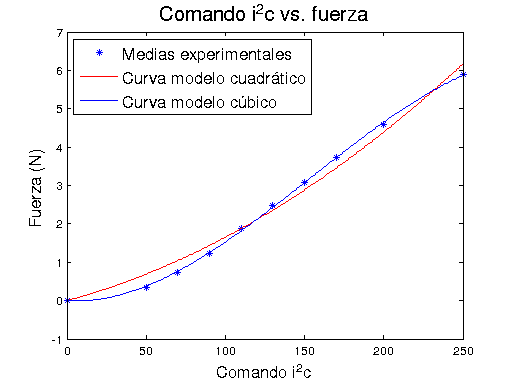
\includegraphics[width=0.7\textwidth]{./pics_motores/if.png}
%  \end{center}
%  \caption{Curva $I^2C$ contra fuerza}
%  \label{fig:if}
%\end{figure}
%Los par\'ametros obtenidos para el modelo cuadr\'atico son:
%	\begin{itemize}
%	\item Par\'ametros $a=5.4588\times 10^{-5}N$,$b=0.0110N$
%	\item Error promedio: $e= -3.712158\times ^{-2}N$
%	\item Desviaci\'on est\'andar: $2.087\times 10^{-1}N$
%	\end{itemize}
%Los par\'ametros obtenidos para el modelo c\'ubico:
%	\begin{itemize}
%	\item Par\'ametros $a\prime=-5.0.166\times 10^{-7}N$,$b\prime=2.3031\times 10^{-4}N$,$c\prime=-0.0028N$
%	\item Error promedio: $e=-1.78\times10^{-3}N$	
%	\item Desviaci\'on est\'andar: $3.71\times 10^{-2}N$
%	\end{itemize}		
%

\subsection{Obtenci\'on de la curva velocidad angular contra torque}

\begin{wrapfigure}{r}{0.6\textwidth}
\vspace{-35pt}
\centering
\subfloat[Curva torque contra velocidad angular]{\label{fig:torque}
  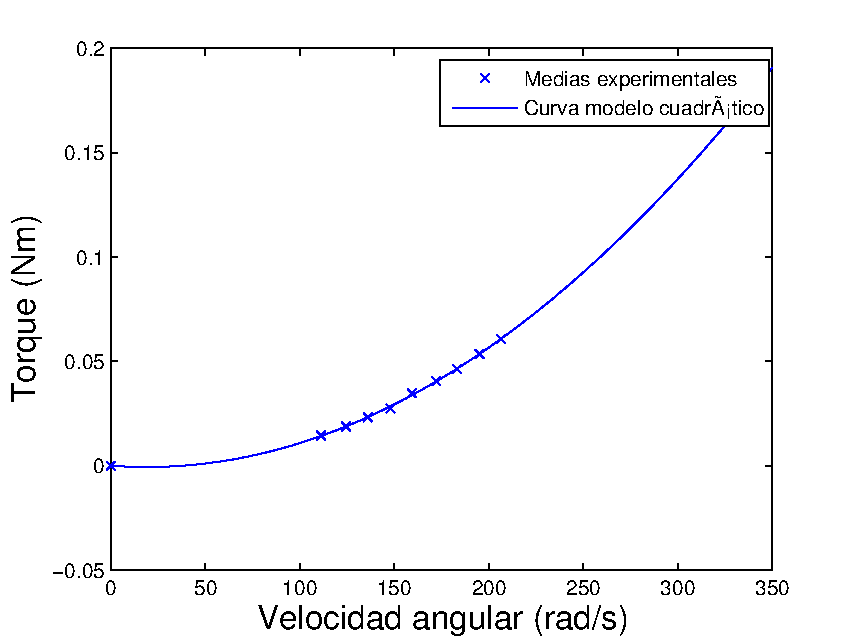
\includegraphics[width=0.6\textwidth]{./pics_motores/torque.pdf}}

\subfloat[Comando $I^2C$, frecuencia y peso]{\label{tab:torque}
\begin{tabular}{|c|c|c|} 
	\hline
	\cellcolor[gray]{0.8} \textbf{$I^2C$} & 
	\cellcolor[gray]{0.8} \textbf{Frec. (Hz)} & \cellcolor[gray]{0.8} \textbf{peso (g)} \\ \hline \hline
	  0 & 0    & 0 \\ \hline
	 50 & 35.4 & -10 \\ \hline
	 55 & 39.6 & -13 \\ \hline
	 60 & 43.3 & -16  \\ \hline
     65 & 47.1 & -19\\ \hline
     70 & 50.7 & -24 \\ \hline
	 75 & 54.8 & -28 \\ \hline
	 80 & 58.3 & -32  \\ \hline
	 85 & 62.1 & -37\\ \hline     
     90 & 65.7 & -42\\ \hline          
\end{tabular}}
\vspace{-10pt}
  \caption{}
\vspace{-85pt}
\end{wrapfigure}

En la tabla \ref{tab:torque} se presentan las medidas obtenidas de velocidad angular y masa medida por la balanza de acuerdo al procedimiento detallado en \ref{sub:torque}.

Recordamos que para la caracterizaci\'on de la respuesta velocidad angular - torque se propuso un modelo cuadr\'atico. Los resultados obtenidos fueron:

\begin{itemize}
 \item Par\'ametros: \newline$a=3.4734\times10^{-6}Nms^2$,\newline$b=-1.3205\times 10 ^{-4} Nms$
\item Error promedio:\newline$\mu = 1.7824\times 10^{-6}Nm$
\item Desviaci\'on est\'andar: \newline$\sigma = 9.2686\times 10^{-4}Nm$ 
\end{itemize}

Si se asume que el error al realizar la medida en el largo del brazo del cuadric\'optero es despreciable, se pueden convertir los errores obtenidos en $Nm$ a gramos.
\begin{itemize}
\item $\mu=0.6265\times10^{-3}g$
\item $\sigma =3.2580\times10^{-1}g$
\end{itemize} 
Tanto el error como la desviaci\'on est\'andar son inferiores en al menos un \'orden que la resoluci\'on de la balanza. En la figura \ref{fig:torque} pueden observarse las medidas experimentales obtenidas y la curva que corresponde al modelo elegido para realizar el ajuste, el resultado es satisfactorio.

\subsection{Respuesta al escal\'on}

En la figura \ref{fig:resp_esc} se muestran las velocidades angulares obtenidas. El tiempo de rise obtenido es de $0.19s$ y la respuesta al escal\'on no presenta pr\'acticamente sobretiro.

\begin{wrapfigure}{l}{0.6\textwidth}
\vspace{-25pt}
  \begin{center}
	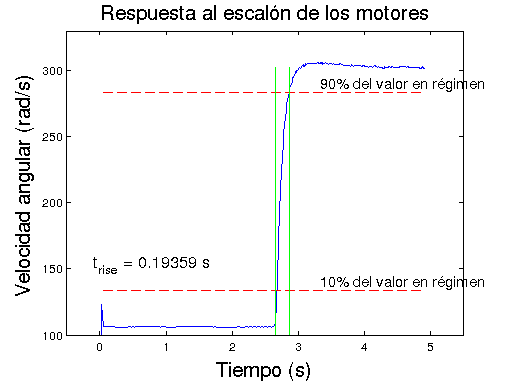
\includegraphics[width=0.6\textwidth]{./pics_motores/resp_esc.png}
  \caption{Curva $I^2C$ contra fuerza}
  \end{center}
  \label{fig:resp_esc}
\end{wrapfigure}

Dado que siempre se trabajar\'a en torno a un valor dado de velocidad angular (ver cap\'itulo \ref{chap:linealizacion}) no se producir\'an variaciones tan abruptas en la velocidad angular de los motores, por lo tanto podemos considerar que los tiempos de respuesta ser\'an mejores que el obtenido en esta prueba, siendo suficientemente r\'apidos como para poder despreciar el transitorio de los motores.

\end{document}